\documentclass[a4paper,11pt]{article}

% ── Packages ──────────────────────────────────────────────────────────────────
\usepackage[T1]{fontenc}
\usepackage[utf8]{inputenc}
\usepackage[english]{babel}
\usepackage[top=2cm, bottom=2cm, left=2.5cm, right=2.5cm]{geometry}
\usepackage{array}
\usepackage{booktabs}
\usepackage{enumitem}
\usepackage{titlesec}
\usepackage{xcolor}
\usepackage{fancyhdr}
\usepackage{graphicx}
\usepackage{hyperref}
\setlength{\emergencystretch}{4em}  % absorb overfull from long \texttt tokens
\usepackage{tikz}
\usetikzlibrary{calc,positioning,shapes.misc}

% ── Colours ───────────────────────────────────────────────────────────────────
\definecolor{erasmusblue}{RGB}{0,82,156}
\definecolor{lightgray}{RGB}{245,245,245}
\definecolor{sectiongray}{RGB}{80,80,80}

% ── Header / Footer ───────────────────────────────────────────────────────────
\pagestyle{fancy}
\fancyhf{}
\renewcommand{\headrulewidth}{0.4pt}
\fancyhead[L]{\small\textcolor{erasmusblue}{Erasmus+ -- Traineeship Certificate (Table D)}}
\fancyhead[R]{\small\textcolor{sectiongray}{Hamza ARIOUICH -- UPV Valencia}}
\fancyfoot[C]{\small\thepage}

% ── Section styling ───────────────────────────────────────────────────────────
\titleformat{\section}[block]
  {\normalfont\large\bfseries\color{erasmusblue}}
  {}{0em}{}[\vspace{2pt}\hrule\vspace{6pt}]

\titleformat{\subsection}[runin]
  {\normalfont\normalsize\bfseries\color{sectiongray}}
  {}{0em}{}[.\quad]

% ── Helper macro ──────────────────────────────────────────────────────────────
\newcommand{\field}[2]{%
  \noindent\textbf{#1:}\quad #2\par\vspace{4pt}}

% ══════════════════════════════════════════════════════════════════════════════
\begin{document}

% ── Title block ───────────────────────────────────────────────────────────────
\begin{center}
  {\Large\bfseries\color{erasmusblue} AFTER THE MOBILITY -- APRÈS LA MOBILITÉ}\\[6pt]
  {\large Table D -- Traineeship Certificate by the Receiving Organisation}\\
  {\normalsize\itshape Tableau D -- Attestation de stage de l'organisme d'accueil}
\end{center}

\vspace{8pt}
\noindent\rule{\linewidth}{0.8pt}
\vspace{6pt}

% ── Administrative fields ─────────────────────────────────────────────────────
\field{Name of the trainee / Nom du stagiaire}{Hamza ARIOUICH}
\field{Name of the Receiving Organisation}{Universitat Politècnica de València (UPV)}
\field{Sector of activity}{Computer Engineering}
\field{Address}{Universitat Politècnica de València, Camí de Vera s/n, Valencia, 46022, Spain -- \url{https://www.upv.es/}}
\field{Start / end of complete traineeship}{08/04/2026 -- 30/07/2026}
\field{Start / end of physical mobility}{08/04/2026 -- 23/07/2026}
\field{Traineeship title}{Integration of a Handwritten Number Recognizer into a Web Application for Exam Management}

\vspace{6pt}
\noindent\rule{\linewidth}{0.4pt}
\vspace{4pt}

% ══════════════════════════════════════════════════════════════════════════════
\section{Detailed Programme of the Traineeship Period}

% ── Gantt timeline ────────────────────────────────────────────────────────────
\begin{center}
\resizebox{\linewidth}{!}{%
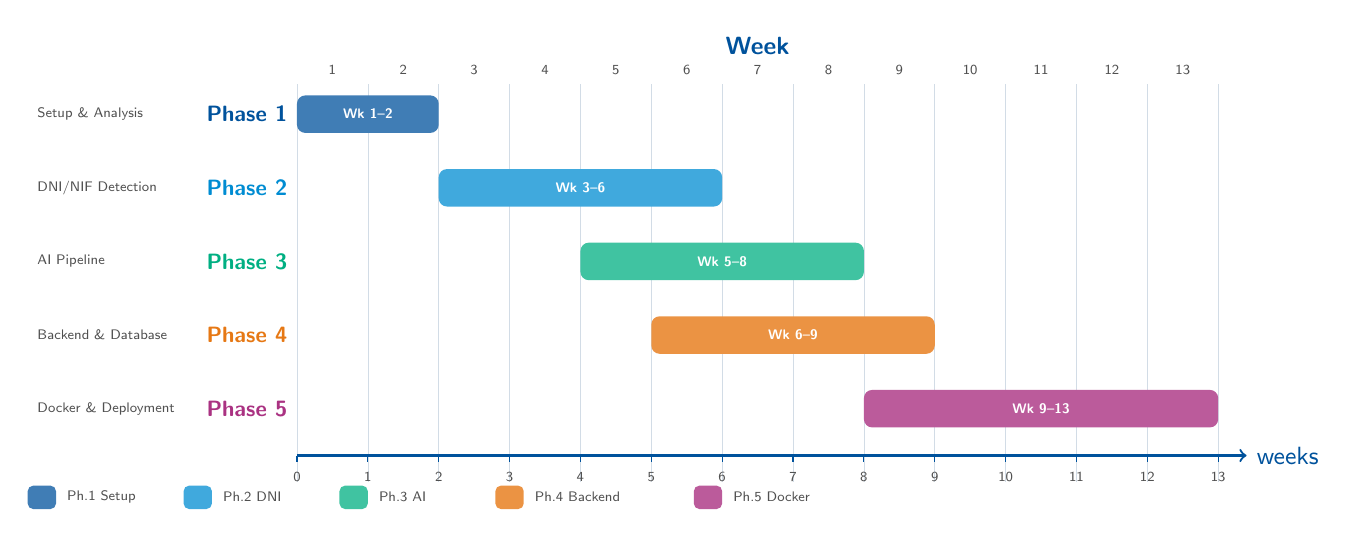
\begin{tikzpicture}[x=0.9cm, y=0.85cm]

  % colours
  \definecolor{c1}{RGB}{0,82,156}
  \definecolor{c2}{RGB}{0,140,210}
  \definecolor{c3}{RGB}{0,175,130}
  \definecolor{c4}{RGB}{230,120,20}
  \definecolor{c5}{RGB}{170,50,130}
  \definecolor{gridcol}{RGB}{210,220,230}

  % ── vertical grid lines (weeks 1–13) ──────────────────────────────────────
  \foreach \w in {0,1,...,13}{
    \draw[gridcol, very thin] (3.8+\w, 0.45) -- (3.8+\w, -5.5);
  }

  % ── week numbers at top ───────────────────────────────────────────────────
  \foreach \w in {1,...,13}{
    \pgfmathsetmacro\xmid{3.8+\w-0.5}
    \node[above, font=\tiny\sffamily, text=sectiongray] at (\xmid, 0.45) {\w};
  }
  \node[above, font=\small\bfseries\sffamily, text=erasmusblue] at (10.3, 0.75) {Week};

  % ── row labels ────────────────────────────────────────────────────────────
  \node[left, font=\footnotesize\bfseries\sffamily, text=c1] at (3.8, 0.0)   {Phase 1};
  \node[left, font=\footnotesize\bfseries\sffamily, text=c2] at (3.8, -1.1)  {Phase 2};
  \node[left, font=\footnotesize\bfseries\sffamily, text=c3] at (3.8, -2.2)  {Phase 3};
  \node[left, font=\footnotesize\bfseries\sffamily, text=c4] at (3.8, -3.3)  {Phase 4};
  \node[left, font=\footnotesize\bfseries\sffamily, text=c5] at (3.8, -4.4)  {Phase 5};

  % ── sub-label (right of row label) ───────────────────────────────────────
  \node[right, font=\tiny\sffamily, text=sectiongray] at (0.0, 0.0)  {Setup \& Analysis};
  \node[right, font=\tiny\sffamily, text=sectiongray] at (0.0, -1.1) {DNI/NIF Detection};
  \node[right, font=\tiny\sffamily, text=sectiongray] at (0.0, -2.2) {AI Pipeline};
  \node[right, font=\tiny\sffamily, text=sectiongray] at (0.0, -3.3) {Backend \& Database};
  \node[right, font=\tiny\sffamily, text=sectiongray] at (0.0, -4.4) {Docker \& Deployment};

  % ── Gantt bars ────────────────────────────────────────────────────────────
  % Phase 1: weeks 1–2   → x from 3.8 to 5.8
  \fill[c1!75, rounded corners=3pt] (3.8, -0.28) rectangle (5.8,  0.28);
  \node[font=\tiny\bfseries\sffamily, text=white] at (4.8,  0.0) {Wk 1--2};

  % Phase 2: weeks 3–6   → x from 5.8 to 9.8
  \fill[c2!75, rounded corners=3pt] (5.8, -1.38) rectangle (9.8, -0.82);
  \node[font=\tiny\bfseries\sffamily, text=white] at (7.8, -1.1) {Wk 3--6};

  % Phase 3: weeks 5–8   → x from 7.8 to 11.8
  \fill[c3!75, rounded corners=3pt] (7.8, -2.48) rectangle (11.8,-1.92);
  \node[font=\tiny\bfseries\sffamily, text=white] at (9.8, -2.2) {Wk 5--8};

  % Phase 4: weeks 6–9   → x from 8.8 to 12.8
  \fill[c4!80, rounded corners=3pt] (8.8, -3.58) rectangle (12.8,-3.02);
  \node[font=\tiny\bfseries\sffamily, text=white] at (10.8,-3.3) {Wk 6--9};

  % Phase 5: weeks 9–13  → x from 11.8 to 16.8 (capped at 16.8)
  \fill[c5!80, rounded corners=3pt] (11.8,-4.68) rectangle (16.8,-4.12);
  \node[font=\tiny\bfseries\sffamily, text=white] at (14.3,-4.4) {Wk 9--13};

  % ── bottom axis ───────────────────────────────────────────────────────────
  \draw[erasmusblue, thick, ->] (3.8,-5.1) -- (17.2,-5.1)
    node[right, font=\small\sffamily, text=erasmusblue] {weeks};
  \foreach \w in {0,1,...,13}{
    \draw[erasmusblue] (3.8+\w,-5.1) -- (3.8+\w,-5.2)
      node[below, font=\tiny\sffamily, text=sectiongray] {\w};
  }

  % ── legend ────────────────────────────────────────────────────────────────
  \fill[c1!75, rounded corners=2pt] (0.0,-5.9) rectangle (0.4,-5.55);
  \node[right, font=\tiny\sffamily, text=sectiongray] at (0.42,-5.72) {Ph.1 Setup};

  \fill[c2!75, rounded corners=2pt] (2.2,-5.9) rectangle (2.6,-5.55);
  \node[right, font=\tiny\sffamily, text=sectiongray] at (2.62,-5.72) {Ph.2 DNI};

  \fill[c3!75, rounded corners=2pt] (4.4,-5.9) rectangle (4.8,-5.55);
  \node[right, font=\tiny\sffamily, text=sectiongray] at (4.82,-5.72) {Ph.3 AI};

  \fill[c4!80, rounded corners=2pt] (6.6,-5.9) rectangle (7.0,-5.55);
  \node[right, font=\tiny\sffamily, text=sectiongray] at (7.02,-5.72) {Ph.4 Backend};

  \fill[c5!80, rounded corners=2pt] (9.4,-5.9) rectangle (9.8,-5.55);
  \node[right, font=\tiny\sffamily, text=sectiongray] at (9.82,-5.72) {Ph.5 Docker};

\end{tikzpicture}%
}% end resizebox
\end{center}

\vspace{4pt}
The trainee worked on \textbf{Madrina}, a full-stack web application that enables university teachers to import,
split, automatically recognise, grade, and redistribute scanned exam papers.
The application relies on two convolutional neural-network (CNN) models: one for reading
handwritten DNI/NIF identity-number characters and one for recognising handwritten grade digits.

\subsection*{Phase 1 -- Codebase analysis and environment setup (weeks 1--2)}
\begin{itemize}[leftmargin=1.5em, itemsep=2pt]
  \item Studied the existing Python AI pipeline, the Node.js/Express backend, and the Angular 13 frontend.
  \item Configured the local development environment: Python virtual environment, MySQL schema
        (\texttt{MargotDB}), Node.js dependencies, and Angular CLI toolchain.
  \item Reviewed the two PyTorch checkpoints (\texttt{best\_model.pt} for DNI recognition,
        \texttt{exammodel4.pt} for grade detection) and their integration as child processes of the backend.
\end{itemize}

\subsection*{Phase 2 -- DNI/NIF detection improvements (weeks 3--6)}
\begin{itemize}[leftmargin=1.5em, itemsep=2pt]
  \item Analysed failure cases in the existing DNI region-of-interest extraction module
        (\texttt{utils/traitement/dni\_processing.py}).
  \item Reworked the character-segmentation and bounding-box logic
        in the coordinate-computation pipeline
        ({\ttfamily compute\_coords\_from\_main\_block})
        to reduce false positives on skewed or low-contrast scan areas.
  \item Improved the Levenshtein-based student-matching logic: tuned the similarity threshold
        (\texttt{MATCH\_RATIO\_THRESHOLD}) and added validation of the reconstructed identifier
        before attempting a database lookup.
  \item Fixed a key-handling bug in the student-roster parsing that caused silent mismatches
        between OCR output and the \texttt{alumnos} table (commit \texttt{f25f34f}).
  \item \begin{sloppypar}Fixed a residual marker-detection regression in the
        copy-boundary detector (\texttt{buscar\_inicio\_copias}),
        introduced during refactoring (commit \texttt{b637bb4}).\end{sloppypar}
\end{itemize}

\subsection*{Phase 3 -- AI model integration and pipeline hardening (weeks 5--8)}
\begin{itemize}[leftmargin=1.5em, itemsep=2pt]
  \item Validated the end-to-end prediction pipeline: PDF ingestion via PyPDF2 and Poppler,
        image extraction, CNN inference with PyTorch on both CPU and CUDA, and structured
        result emission over stdout (\texttt{progress}, \texttt{new-calificado}, \texttt{done}).
  \item Introduced a \texttt{validate\_runtime()} check at startup to detect missing model
        checkpoints or malformed student-roster arguments before any page is processed.
  \item Added parallel preprocessing using \texttt{ProcessPoolExecutor} to distribute
        coordinate-computation work across available CPU cores.
  \item Translated all in-code comments and documentation from Spanish/French to English
        (commit \texttt{32f17a3}) to improve maintainability for international contributors.
\end{itemize}

\subsection*{Phase 4 -- Backend and database work (weeks 6--9)}
\begin{itemize}[leftmargin=1.5em, itemsep=2pt]
  \item Extended the Node.js/Express Data Access Layer (\texttt{DAL.js}) with new SQL queries
        against the \texttt{MargotDB} MySQL schema (tables: \texttt{usuarios}, \texttt{asignaturas},
        \texttt{alumnos}, \texttt{examenes}, \texttt{calificados}).
  \item Reviewed and validated the session-token authentication interceptor applied to all
        \texttt{/api} routes.
  \item Contributed to Socket.IO event handling (\texttt{examen-predict},
        \texttt{examen-predict-kill}) to ensure real-time progress updates reach the Angular
        frontend reliably.
  \item Verified PDF-to-image conversion orchestration (Poppler \texttt{pdftoppm},
        \texttt{pdfseparate}, \texttt{pdfunite}) and ZIP archive generation (\texttt{archiver}).
\end{itemize}

\subsection*{Phase 5 -- Dockerisation and production deployment (weeks 9--13)}
\begin{itemize}[leftmargin=1.5em, itemsep=2pt]
  \item Wrote and refined \texttt{Dockerfile.backend} and the Angular \texttt{Dockerfile} so that
        the backend (Node.js + Python AI module) and the frontend (Nginx-served static build)
        run as separate Docker services.
  \item Authored \texttt{docker-compose.yml} (development) and \texttt{docker-compose.prod.yml}
        (production) orchestrating the frontend, backend, and MySQL containers with
        environment-variable injection and named volumes for persistent data.
  \item Supported an external database configuration option in \texttt{docker-compose}
        (commit \texttt{16faafe}), allowing the application to connect to an existing
        MySQL server rather than spinning up a container.
  \item \begin{sloppypar}Wrote comprehensive deployment documentation
        (\texttt{README\_deploy.md}, \texttt{README\_deploy\_prod.md}):
        Nginx reverse-proxy configuration, Socket.IO upgrade headers,
        TLS, systemd service creation, and backup/restore procedures.\end{sloppypar}
  \item Performed end-to-end validation of the Dockerised stack: account creation, exam upload,
        AI prediction, manual correction, and ZIP export.
\end{itemize}

% ══════════════════════════════════════════════════════════════════════════════
\section{Knowledge, Skills and Competences Acquired}

\subsection*{Technical knowledge}
\begin{itemize}[leftmargin=1.5em, itemsep=2pt]
  \item Deep understanding of convolutional neural networks applied to optical character recognition
        (handwritten digit and alphanumeric string recognition with PyTorch).
  \item Knowledge of image-processing techniques: bounding-box extraction, contrast normalisation,
        region-of-interest cropping with OpenCV and NumPy.
  \item Understanding of the full software stack of a modern web application:
        relational database (MySQL), REST/WebSocket backend (Node.js, Express, Socket.IO),
        and single-page application frontend (Angular, TypeScript, RxJS).
  \item Practical knowledge of Docker and Docker Compose for multi-container application
        packaging, Nginx reverse-proxy configuration, and production deployment on Linux servers.
\end{itemize}

\subsection*{Practical skills}
\begin{itemize}[leftmargin=1.5em, itemsep=2pt]
  \item Ability to diagnose and fix bugs in an AI inference pipeline by combining log analysis,
        manual testing with sample PDFs, and controlled unit experiments.
  \item Proficiency in SQL query writing and optimisation within a Node.js DAL pattern.
  \item Skill in writing production-grade \texttt{docker-compose} configurations including
        secret management via \texttt{.env} files, health checks, and volume mapping.
  \item Experience writing clear technical documentation in English for an international audience.
\end{itemize}

\subsection*{Transversal competences}
\begin{itemize}[leftmargin=1.5em, itemsep=2pt]
  \item Ability to read and extend a pre-existing multi-language, multi-technology codebase.
  \item Autonomous problem-solving and debugging in an international research environment.
  \item Version-control discipline: meaningful commit messages, feature branches, and pull-request
        workflow on GitHub.
  \item Adaptability to a Spanish-language academic environment and to the working culture of
        the Universitat Politècnica de València.
\end{itemize}

% ══════════════════════════════════════════════════════════════════════════════
\section{Evaluation of the Trainee}

The trainee, Hamza ARIOUICH, demonstrated a high level of technical competence and professional
commitment throughout the internship period.

\begin{itemize}[leftmargin=1.5em, itemsep=4pt]
  \item \textbf{Quality of work:} The contributions delivered were correct, well-structured, and
        aligned with the project's coding conventions. Bug fixes were accompanied by root-cause
        analysis and targeted tests.
  \item \textbf{Autonomy and initiative:} The trainee took ownership of complex tasks (DNI
        detection improvement, full Dockerisation) with minimal supervision, proposing and
        implementing solutions independently.
  \item \textbf{Adaptability:} The trainee efficiently navigated a heterogeneous codebase
        spanning Python, JavaScript/TypeScript, SQL, and shell scripting, and quickly became
        productive in an unfamiliar academic environment.
  \item \textbf{Communication and documentation:} Technical documentation was produced in clear,
        professional English. The trainee communicated progress and blockers effectively to the
        supervising team.
  \item \textbf{Overall assessment:} Excellent. The trainee's contributions materially improved
        the reliability and deployability of the Madrina application and are integrated into the
        production branch.
\end{itemize}

\vspace{20pt}

% ── Signature block ───────────────────────────────────────────────────────────
\noindent
\begin{tabular}{@{}p{0.45\linewidth}@{\hspace{0.08\linewidth}}p{0.45\linewidth}@{}}
  \textbf{Date:} \dotfill &  \\[30pt]
  \multicolumn{2}{@{}l@{}}{\textbf{Name, signature and stamp of the Supervisor at the Receiving Organisation:}} \\[40pt]
  \dotfill & \\
\end{tabular}

\end{document}
